

\section{Results}

\subsection{Position dependence}

Figure \ref{fig:pos_dependence_aes} shows the position dependence of the AES signal. 

\begin{figure}[h]
    
\includegraphics[width=0.8\linewidth]{\repodir/final/figures/output/Fig3_Position_AES.png} 
    \caption{Position dependence of atomic potassium as measured by AES and predicted by CFD. The CFD data is sampled along a line on the torch axis, either directly on the torch axis or offset perpindicular to simulate misalignment in the AES beam. }
    \label{fig:pos_dependence_aes}
\end{figure}

We now examine the position dependence of the MWS signal in figure \ref{fig:pos_dependence_mws}.  These measurements are used to motivate the choice of position for the Kwt dependence measurements presented in the next section. 

We observe that near the exit of the torch there is a significant fluctuation in the MWS signal in the absence of a laser pulse. The temperature at the exit of the torch is sufficiently high for thermally induced conductivity. Variations in the flow or potassium distribution could cause these time dependent fluctuations. We provide some analysis of these background fluctuations in the SI (TODO).

For the present discussion, the important point is that these fluctuations are significant compared to the signal induced by the laser pulse, and they therefore preclude accurate measurement of the time decay of the AS signal. 

In Figure \ref{fig:pos_dependence_mws}B the we quantify the signal to fluctuation ratio to find the optimal position for the MWS diagnostic. We define the signal as the maximum of $AS$ ($AS_{max}$) within a microsecond of the laser pulse, and the fluctuation as the standard deviation of $AS$ in the time prior to the laser pulse ($PP_{std}$). We observe that both $AS_{max}$ and $PP_{std}$ increase until about 100 mm downstream from the torch, and then decrease. However, $PP_{std}$ decreases more rapidly than $AS_{max}$, so the signal to fluctuation ratio increases to a maximum at approximately 180 mm downstream from the torch. 


\begin{figure}[h]
    
\includegraphics[width=0.8\linewidth]{\repodir/final/figures/output/Fig4_Position_MWS.png} 
    \caption{Position dependence of the MWS signal. The data are taken for full laser power and 1\% nominal K mass fraction. All error bars are standard deviation across Runs. A) AS profiles taken at 104.8 mm downstream of the barrel exit The hue represents different repeats of the test case sequence, with each line being an average of all oscilloscope acquisitions in a given test case.  B) The AS signal further downstream at the nominal position of 178 mm. C)  The maximum of the AS signal within 1 $\mu s$ of the laser pulse (0 $\mu s$). The change in potassium photodiode with laser pulse is also shown. The photodiode data for the nominal test case was only obtained on 2024-05-24, but comparisons between the AS and PD signals for different equivalence ratios are presented in the SI. D) The ratio of the Max AS and pre-pulse magnitude statistics. For B, C, and D the confidence intervals represent the standard deviation across runs. } 
    \label{fig:pos_dependence_mws}
\end{figure}





Together the position (Figure \ref{fig:pos_dependence_mws}) and the power dependence (Figure S\ref*{fig:SI_power_dependence}) motivate the conditions used for the Kwt dependence presented below: Measurements are taken at 178 mm downstream of the barrel in order to maximize the signal to fluctuation ratio and accurately measure the profile of the AS decay after the laser pulse. We note, as discussed further later, that the AS decay rate does not appear to depend sensitively on the position (see \ref{fig:pos_dependence_mws} and SI). We take measurements at full laser power (~7 mJ) to maximize the signal and as the exponential time constant does not appear to depend sensitively on the laser power

\clearpage

\subsection{K dependence}

Figure \ref{fig:kwt_ionization} shows results with the mobile setup positioned at 178 mm and full laser power. 

\begin{figure}[h]
    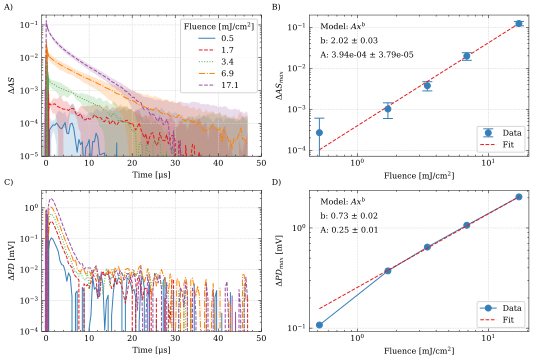
\includegraphics[width=0.8\linewidth]{\repodir/final/figures/output/Fig5_Kwt_Ionization.png} 
    \caption{Kwt dependence: Measurements and predictions at the goldilocks zone (Goldi) and full laser power as a function of nominal potassium weight percent A) species number density results and CFD predictions. Goldi = Goldilocks. B) MWS AS maximum (within 1 us of laser pulse) and photodiode signal. The photodiode signal is from the K filtered photodiode and is the difference between the maximum of the signal in time and the signal 1 us before the laser pulse. C) Decay time constant. The time constant is measured experimentally through and exponential fit of the AS signal. The CFD predictions are based on collision assisted termolecular recombination rates as discussed in the text. }
    \label{fig:kwt_ionization}
\end{figure}



Figure \ref{fig:kwt_recombination} shows analysis of the $\Delta AS$ decay measurmeents.  Figure \ref{fig:kwt_recombination}A shows the $\Delta AS$ time profile for a range of K mass fraction. Immediately after the laser pulse, there is a region of of changing slope in the logarithm of the $\Delta AS (t)$ profile. After a few microseconds, the profile becomes an exponential decay. Assuming, $\Delta AS (t) \propto \Delta n_e (t)$, where $\Delta n_e (t)$ is the time dependent change in the free electron density from the steady state concentration, we derive in the SI a differential equation for the decay of $\Delta n_e (t)$. In the regime where $\Delta n_e (t)$ is small, the equation has the exponential form.  

\begin{equation}
    \label{eq:fit_eq}
    \frac{d\Delta n_e (t)}{dt} = - k_{r, m, eff} \Delta n_e (t) 
\end{equation}

The time constant of the exponential decay for capture with species X, $\tau$, is given by

\begin{equation}
    \label{eq:tau_krm}
    k_{r, m, X} = \frac{1}{\tau} = k_{r, b, X}n_{X,0}
\end{equation}

Where, $\tau$ is the exponential time constant and $n_{X,0}$ is the equilibrium species concentration of X, and $k_{r, b, X}$ is the bimolecular recombination rate coefficient for capture by X. The fitted time constants are shown in Figure \ref{fig:kwt_recombination}B.


\begin{figure}[h]
    
\includegraphics[width=0.8\linewidth]{\repodir/final/figures/output/Fig6_Kwt_Recombination.png} 
    \caption{Kwt dependence: Measurements and predictions at the goldilocks zone (Goldi) and full laser power as a function of nominal potassium weight percent A) species number density results and CFD predictions. Goldi = Goldilocks. B) MWS AS maximum (within 1 us of laser pulse) and photodiode signal. The photodiode signal is from the K filtered photodiode and is the difference between the maximum of the signal in time and the signal 1 us before the laser pulse. C) Decay time constant. The time constant is measured experimentally through and exponential fit of the AS signal. The CFD predictions are based on collision assisted termolecular recombination rates as discussed in the text. }
    \label{fig:kwt_recombination}
\end{figure}



We calculate expected decay constants for electron capture by various species in \ref{fig:kwt_dependence}C to compare to the experimental decay constant. The expected decay constants are calculated through equation \ref{eq:tau_krm} with $n_{X,0}$ given by the CFD results at the goldilocks position. 

We have searched for data on reaction kinetics that are compatible with first-order recombination of electrons (eq. \ref{eq:fit_eq}). For some reactions and $k_{r,b,X}$ is given directly in the literature in units of $cm^3/s$. Some reactions are termolecular and further depend on a collisional partner, M, and are of the form [X] +[e-] + M \rightarrow [X-] + M. in this case $k_{r,b} = k_{r,tm} [M]$, where $k_{r,tm}$ is the termolecular recombination rate given in units of $cm^6/s$ and [M] is the number density of the collision partner.  The densities of [M] and [X] are taken from the CFD results at the goldilocks position.

We find the following reactions with kinetic data available in the literature(T in K):

\begin{itemize}
    \item K+ + e- + M \rightarrow K + M : $4e-24 T^{-1} cm^3/s$ T(Jensen 1978) 
    \item O2 + e- + M \rightarrow O2- + M : Variable (Axford 1997 and Goodings 1979)
    \item OH + e- + M \rightarrow OH- +M  $3e-31 cm^6/s$ (Axford 1997)
    \item H2O + e- \rightarrow H2O- $1.6e-5 exp(36060/T) cm^3/s$ (Axford 1997)
\end{itemize}

For the OH and K capture reactions, we use the number density of the entire flame as the collisional partner. 

For recombination with molecular oxygen, there is significant uncertainty in the rate constant and we consider a few possibilities indicated in the legend of \ref{fig:kwt_dependence}C. Axford 1997 discussed this uncertainty and presented a range of rate constants ultimately deciding on a value of $5e-31 cm^6/s$ for their H2 + O2 + N2 flame, which we consider as '$O2_A$' using the number density of all species as the collisional partner density. In the same discussion they specify the dominant collisional partners of the various literature values of the rate constant, so for '$O2_B$' we preform a sum of species dependent $k_{r,tm}$ with the CFD number densities for each collisional partner to determine an overall $k_r$. The constants presented by Axford 1997 include low temperature measurements, but mention that $k_{r,th}$ is expected to decrease at flame temperatures. Goodings 1979 found a much lower rate constant for similar flames and speculated a large negative temperature coefficient for the oxygen capture reaction. We consider this as '$O2_C$' and use the number density of all species as the collisional partner density. It is not clear why Axford 1997 did not mention the Goodings 1979 result (Hayhurst was on both papers). 

In summary there is a large uncertainty in the $k_{r,th}$ for the oxygen capture reaction. We present a range of predictions in \ref{fig:kwt_dependence}C. Our results fall within this large deviation. All other reactions predict decays much longer than the observed expermental decay. 

We note that the previously mentioned sources have much better agreement on the OH, H2O, and K capture reactions than the O2 capture reactions. 



